\chapter{System Design}
\section{Overview}
\begin{figure}[h]
\centering
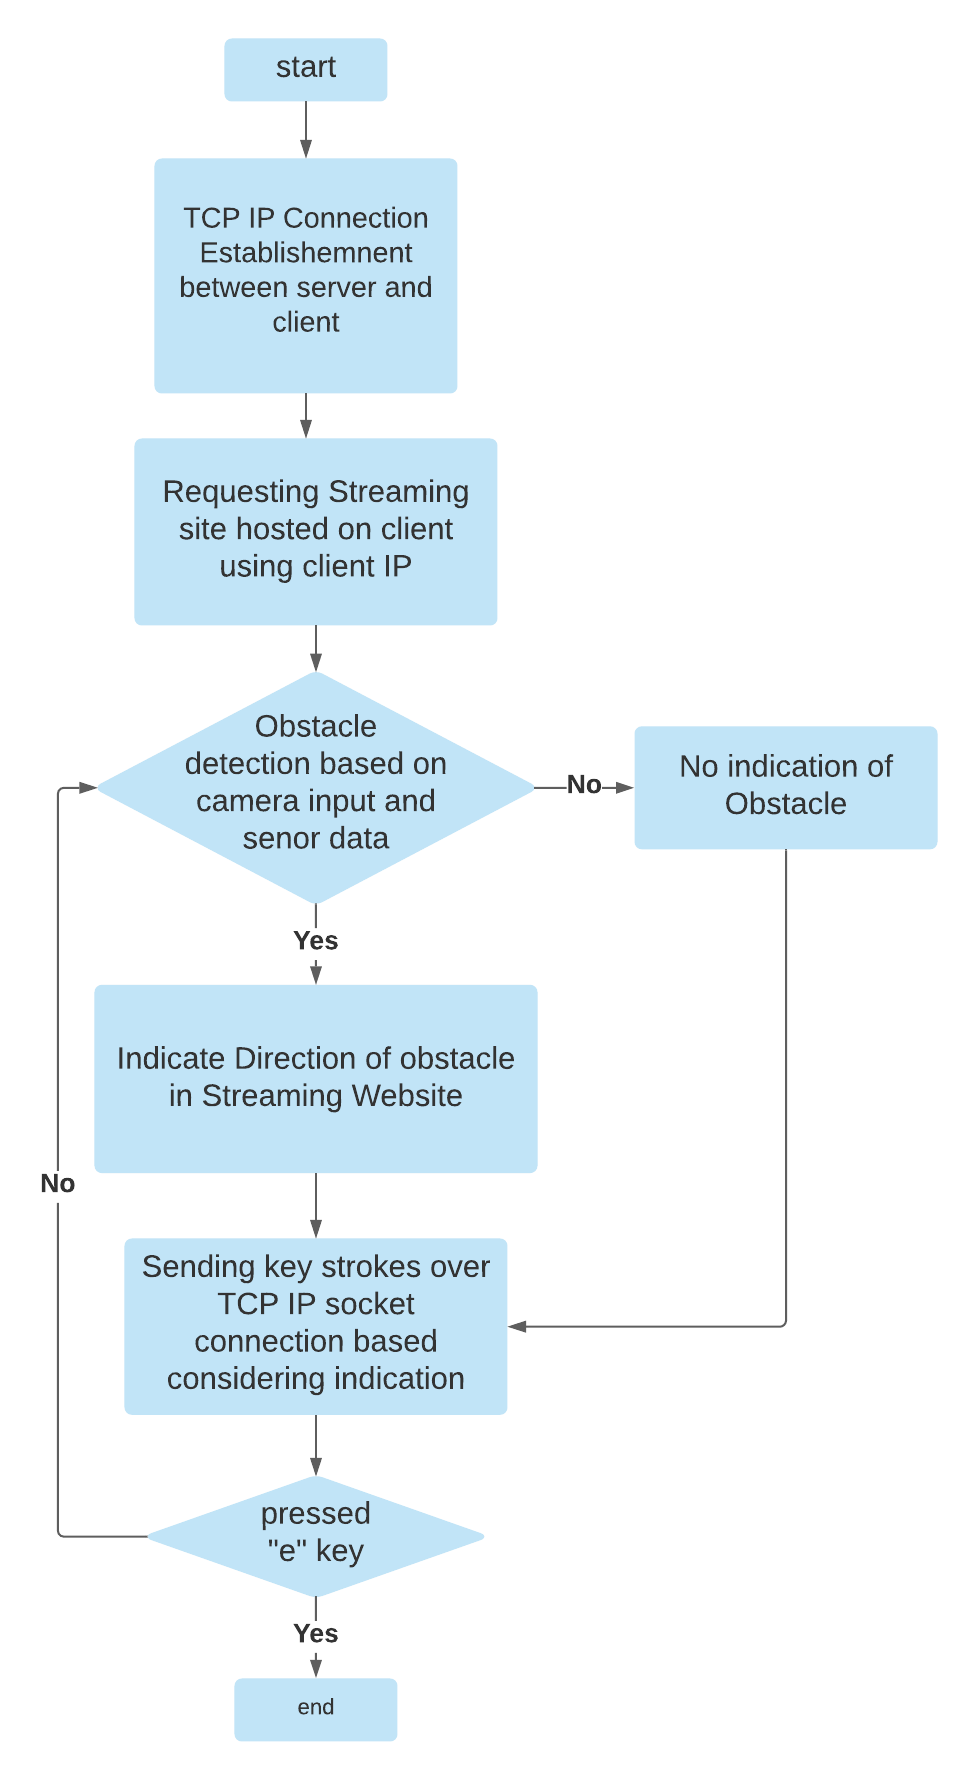
\includegraphics[scale=0.25] {project_flowchart.png}
\caption{System Design Flowchart}
\end{figure}
The above flowchart describes the overall design of the wireless communicated robot
movement and the web application working for the live feed from camera mounted
on the robot. As we already know the hardware and software components used we
will further go ahead and discuss the system design that we developed.
\section{Designing the Web Application}
\paragraph{}Web technologies we are using for the project are HTML, CSS, Bootstrap, Python and Flask. These technologies are needed to configured in a proper manner for the web application to work properly. In the directory where the project folder for the web application is established all the constituent files and folders have to be kept in a specific format as supported by Flask.

\begin{figure}[h]
\centering
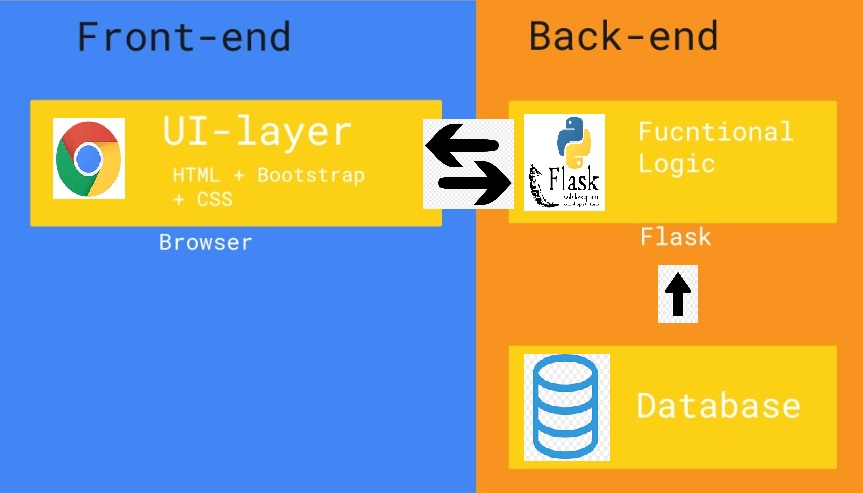
\includegraphics[scale=0.4]{bdweb.jpg}
\caption{Block Diagram of Web Application}
\end{figure}

\subsubsection*{Here is the basic file structure for flask:} 
\texttt{\textbf{\small{yourapp/}}}

\texttt{\small{.py}}

\textbf{\texttt{\small{static/}}}

\hspace{0.5in}\texttt{\small{.js}}

\hspace{0.5in}\texttt{\small{.css}}

\hspace{0.5in}\texttt{\small{Images}}

\textbf{\texttt{\small{templates/}}}

\hspace{0.5in}\texttt{\small{.html}}

\subsubsection*{Description of files:}
\textbf{.py}: contains the actual python code that will import the app
and start the \\development server.\\
\textbf{static/} : contains static files i.e. CSS (including bootstrap), JavaScript, images.\\
\textbf{templates/} : This is where you store your HTML templates
i.e. index.html, \\layout.html\\
Python modules used in app.py (main web app Script/Program):
\begin{enumerate}[1.]
\item Flask - Web application framework
\item CV2 - Library to help the drawing process with Open-CV
\item Sockets - provides access to the BSD socket interface
\item Keyboard - provides various keys-related functions
\item Time - provides various time-related functions
\item Rpi.GPIO - This package provides a class to control the GPIO on a Raspberry Pi.
\end{enumerate}

\section{Designing the remote controlled robot movement}
The heart of the robot is a raspberry pi 4(2GB RAM) which is a credit card sized computer used in a wide range of applications varying from a simple personal \\computer to advanced robotics.  The Raspberry Pi has an inbuilt Wi-Fi module which can connect to any network. The OS of the Raspberry Pi resides within an SD card of size 32 GB. The motors of the robot are controlled using the PWM pins available on the 40 pin GPIOS of the Raspberry Pi. The Raspberry Pi GPIO pins output a \\current insufficient to drive the motors and hence we have used the L298N motor driver which amplifies the current so that it drives the motors easily. In order to get \\information about the surroundings of the area in which the robot is patrolling we have used three sensors. They are ultrasonic sensors, Picamera v2.1 and a USB mic. The ultrasonic sensor is used to measure distances on all sides of the robot in order to ensure that the robot doesn’t collide with any obstacles in its vicinity. The Picamera acts as the eyes of the robot. The robot is steered using the ‘a’, ’w’, ‘s’ and ‘d’ keys of the robot based on the camera feed received.
\vspace{0.1in}
\begin{figure}[h]
\centering
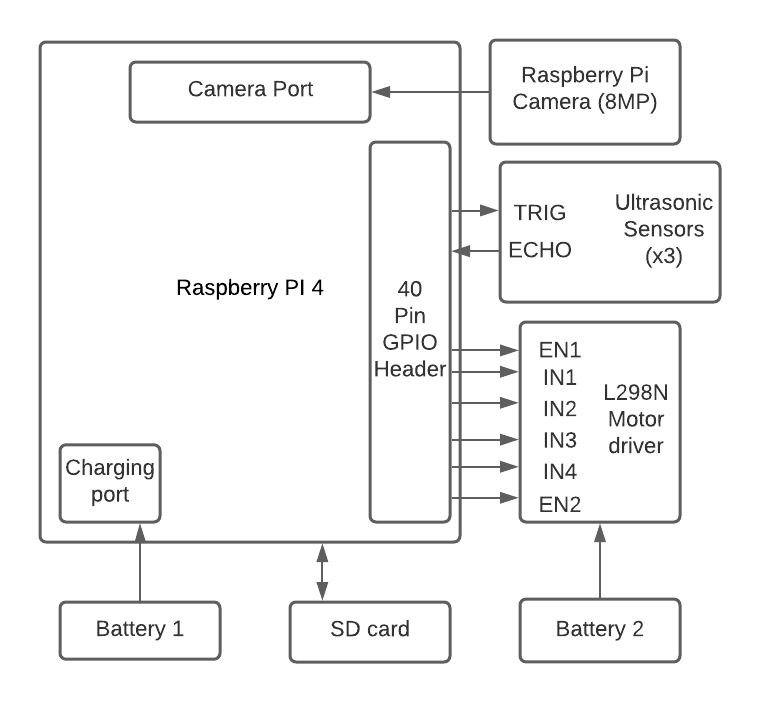
\includegraphics[scale=1]{Block_diagram.png}
\caption{Block Diagram of Robot}
\end{figure}
\section{TCP/IP Communication}
%The communication protocol which we have opted to use in our project is the TCP/IP socket protocol.  The TCP/IP socket protocol establishes a peer-to-peer connection between the server and the client followed by which data is transferred in the form of packets of fixed length. In our case each packet is 1024 bytes in length. A socket is one end of a 2-way communication. A socket consists of an IPV4 address and a port number. The connection between the server and the client happens with a series of events occurring on both the server and the client sides.
%\subsubsection*{The following occurs on the server side:} 
%\begin{enumerate}[1.]
%\item Declaration of the socket object: first a socket object is created which is an \\instance of the socket class.
%\item Socket binding: The process of assigning a port number to a socket is called socket binding.  
%\item Listening for connections: Once the socket has been binded it soon starts listening for connection requests from active clients. 
%\item Accepting Client connections: The server accepts all the client connections who are willing to connect to the server. Upon connection the server receives \\connection objects using which the server sends data to the client.
%\item Data transfer: The server uses the connection objects to send data to the client.
%\end{enumerate}
%\subsubsection*{The following occurs on the client side:}
%\begin{enumerate}[1.]
%\item Declaration of the socket object: first a socket object is created which is an \\instance of the socket class.
%\item Connection: The client sends a connection request to the server using the ip and port number of the server. 
%\item Data transfer: Once the server accepts the connection of the client, the client starts receiving the data sent by the server.
%\end{enumerate}
A TCP-IP Socket is a combination of a computer's IP address and port number. The IP address is used to identify a computer in the network while the port number distinguishes between the various applications running on the computer.\\ Port numbers range from 0-65535 and are divided into the following ranges:
\begin{enumerate}
\item[a.] 0-1023: Allocated to server services. Example SMTP uses 25 as the port number
\item[b.] 1024-49151: This can be registered for services but cannot run user defined programs
\item[c.] 49151-65535: These can be used freely for client programs
\end{enumerate}
TCP-IP sockets provides an easy way to link two computers for data transfer. It is easy and quickly configurable. It provides bidirectional data transfer and ensures that the sequence of data being transferred is maintained thereby ensuring real timeliness.\\
The two devises which we have used in our project are a Raspberry Pi and any PC/Laptop of any kind. The PC/Laptop is the server while the Raspberry Pi is the client and is the heart of the robot. The key strokes are recorded using a python library called keyboard and this information is sent to the Raspberry Pi over sockets.\\
The following events occur during the data transfer in the server and the client:
\begin{enumerate}
\item Server side:
\begin{enumerate}
\item[a.] Socket object declaration: In order to access the socket functionality firstly a Socket object of the class Socket from the Python3 Socket library is declared.
\item[b.] Socket binding: Socket binding is the process of assigning an IP address a port number.
\item[c.] Listening for client connection requests: The server now begins to listen to active clients for connection requests. The number of connections to be accepted can be specified
\item[d.] Accepting client connections: The server begins to accept client connections and for every client connection accepted the server receives a connection object and a tuple. The tuple consists of the clients IP address and Port number.
\item[e.] Data Transfer: The server now enters an infinite while loop where it waits for keys of the PC/Laptop to be pressed. The information to be sent is firstly encoded from string to byte string and is then sent over socket to the client. Once a key is pressed the keystroke is recorded as a String, converted to byte string and is then sent. If no key is pressed then a default value is sent in the same way as mentioned above to prevent timeout.
\end{enumerate}
\item Client Side: 
\begin{enumerate}
\item[a.] Socket object declaration: In order to access the socket functionality firstly a Socket object of the class Socket from the Python3 Socket library is declared.
\item[b.] Connection to the server: The client uses the connect function of the socket to send a connection request to the server using the servers IP address and Port number
\item[c.] Data Transfer: Once the server accepts the client's connection request the client begins to receive data sent by the server in the form of chunks. The chunk size can be specified. The received chunk of data is decoded back into string and based on the final string the appropriate action is performed by the robot using an if-else-if ladder.
\end{enumerate}
\end{enumerate}
\section{Sensor Data API}
In this part of the project we made an API which interacts with an ultrasonic distance sensor using the raspberry pis GPIO header. We use three 
sensors,one for the left, one for the right and one for the back of the car. The api acquires the sensor data and it is returned in the JSON format. 
Using JavaScript and jQuery we request the data from the API and change the content on the screen using DOM manipulation.
\begin{figure}[h]
\centering
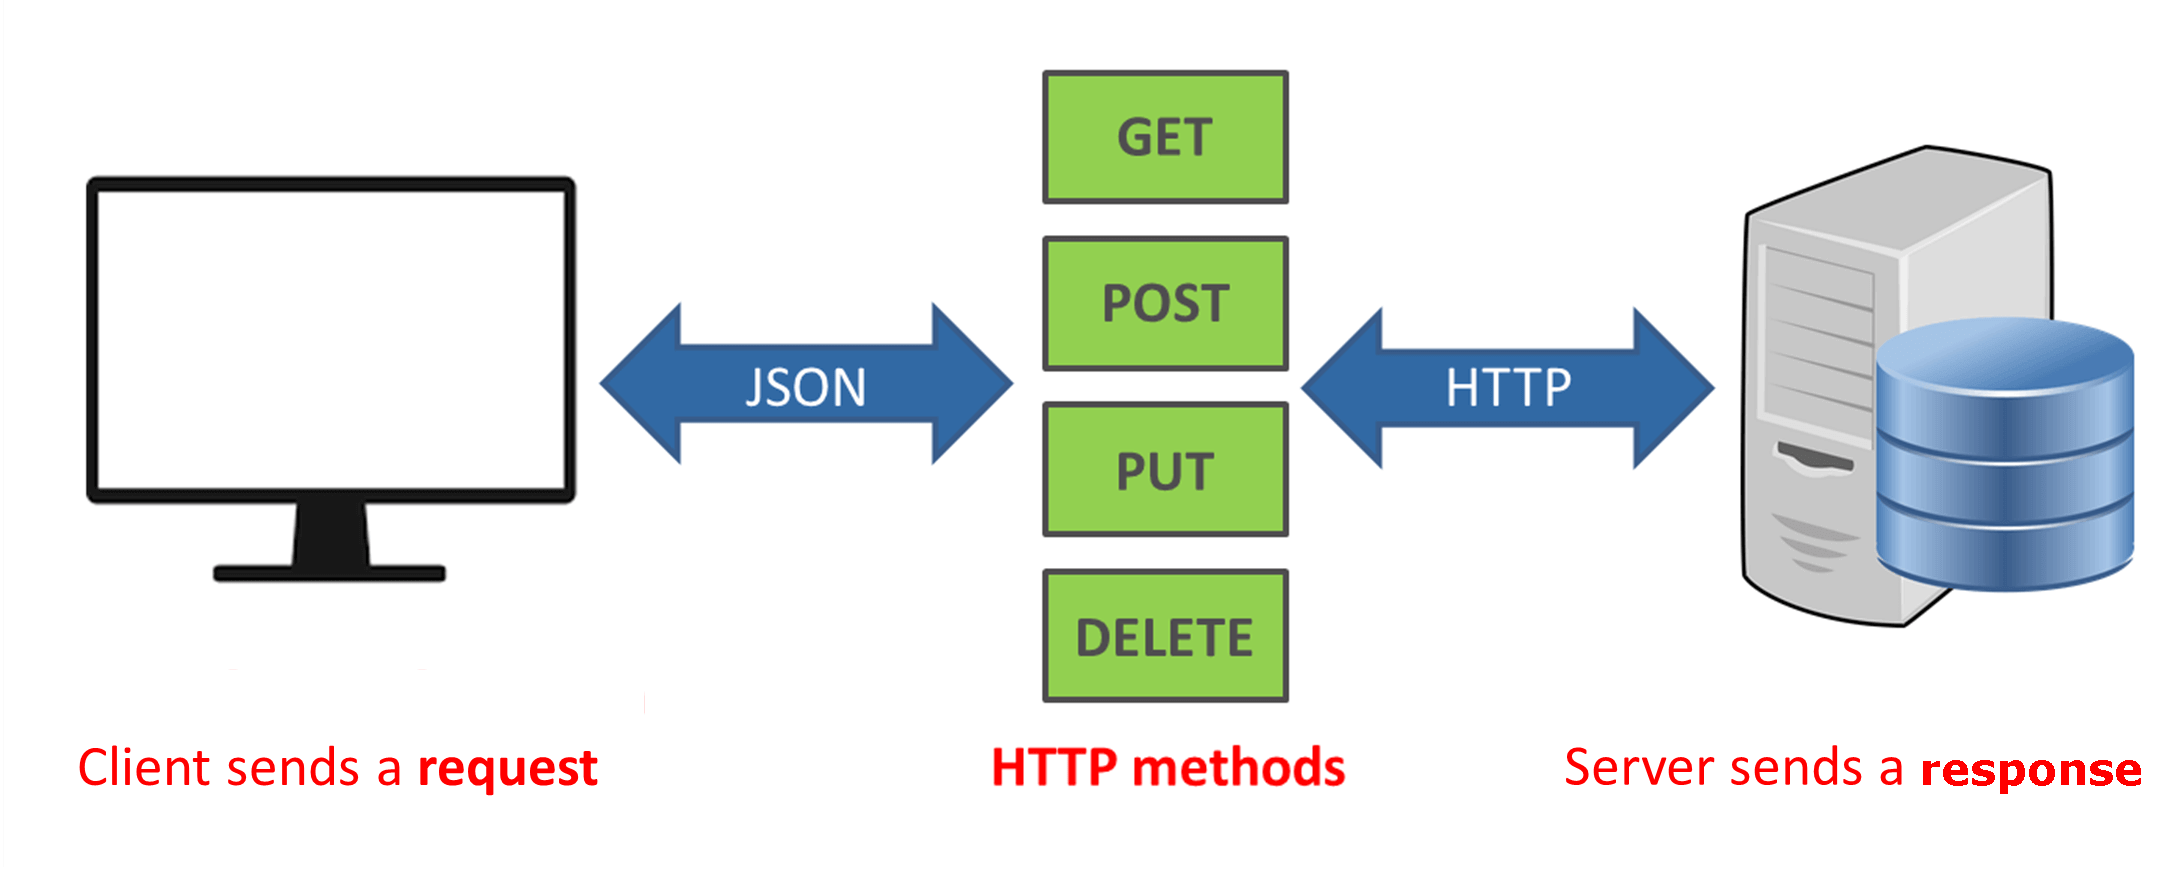
\includegraphics[scale=0.1]{api.png}
\caption{Working of API(Local)}
\end{figure}
\subsubsection*{RESTful API}
REST stands for representational state transfer and the APIs which follow this architecture are called RESTful APIs. A REST API is a software architecture 
style which uses a subset of the HTTP protocol. An API maybe viewed as a bridge between two entities, an information provider and an information user. 
The 5 methods used in a RESTful API are GET, POST, PUT, DELETE, PATCH.
In our project we make use only of the GET method.\\
GET: Used to retrieve data from a server. Upon retrieving the data successfully the error code given is 200(OK). If the resource is not found the error code is 404 (NOT FOUND) and if the request sent is not properly formatted then the error code is 400(BAD REQUEST).A response maybe in the form of a HTML code, JSON or XML.

\section{Ultrasonic Sensor Circuit}
The output of the Ultrasonic sensor (HSCR-04) is 5V while the maximum input voltage acceptable by the Raspberry Pi is 3.3V. If the output of the ECHO pin is not stepped down to 3.3V then the Raspberry Pi can get damaged.
Thus we need to step down the voltage using a voltage divider resistor network. Circuit is show above and the calculation for it as follows:

\begin{small}
$$V_{out} = V_{in} * \frac{R_2}{R_1 + R_2}$$
$$3.3 = 5 * \frac{R_2}{680 + R_2}$$
$$R_2 = 1320 \Omega$$
$$R_2 \approx 1560 \Omega$$
\end{small}
\begin{figure}[h]
\centering
\includegraphics[scale=0.6]{Ultracircuit.png}
\caption{Ultrasonic Circuit}
\end{figure}
\vspace{0.1in}
\section{Solar Charging}
\begin{figure}[h!]
\centering
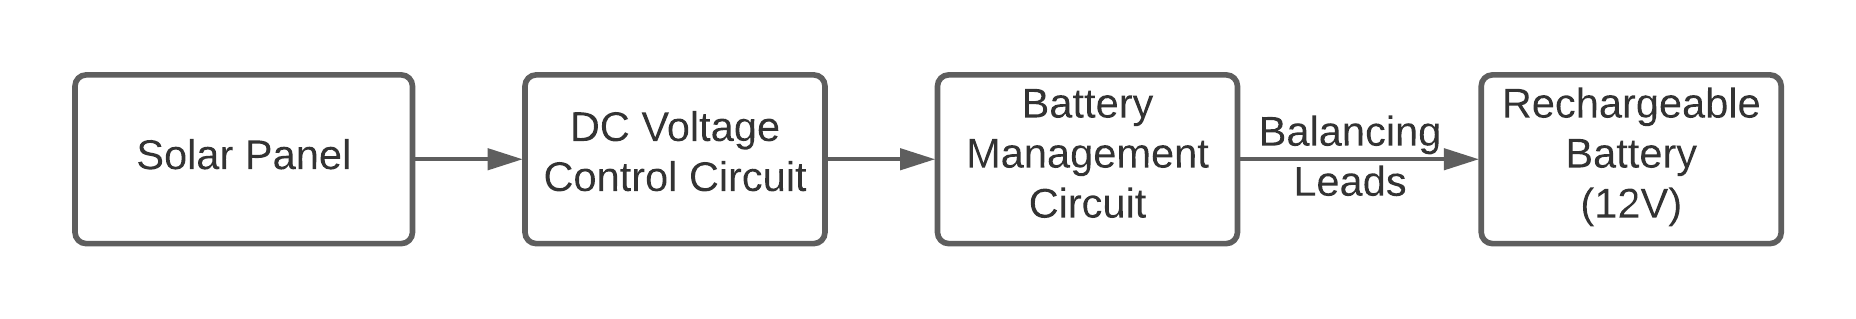
\includegraphics[scale=0.9]{Solarbd.png}
\caption{Block Diagram of Solar Charging Circuit}
\end{figure}
The above Fig. 6 represents the  block diagram of various components used in the Solar Charging circuit.
\begin{enumerate}
\item[a.] \textbf{Solar panel}: It is the input source for the circuit. It provides voltage between 0-26V.
\item[b.] \textbf{DC Voltage Control Circuit}: It helps regulate the fluctuating output voltage of the solar panel varying from 0-26V to Constant Voltage(CV) of 12V(For 12V Li-Po Battery).
\item[c.] \textbf{Battery Management System}: This circuit prevents Short Circuit, Over Charging and also helps in faster charging. 
\end{enumerate}

%\subsection{GIX algorithm}
%The GIX algorithm is an acronym for “Gone in exchange” Algorithm . The GIX algorithm ensures that data is transferred securely over the internet by using \\encryption and decryption algorithms on the sender and the receiver sides \\respectively.
%\subsubsection*{The following occurs on the sender side: }
%\begin{enumerate}
%\item First the pure control message is received. Which in our case is the key pressed.
%\item A random key is chosen and the control message is encrypted using the key.
%\item The random key is hidden within the encrypted control message and the final encrypted message is returned.
%\item The encrypted message is sent over the internet.
%\end{enumerate}
%\subsubsection*{The following occurs on the receiver side: }
%\begin{enumerate}
%\item The encrypted control message is received. 
%\item The hidden key is found within the encrypted message.
%\item Using the key, the message is decrypted to get the pure control message.
%\item Appropriate tasks are performed based on the control message received. 
%\end{enumerate}
%\begin{figure}[h]
%\centering
%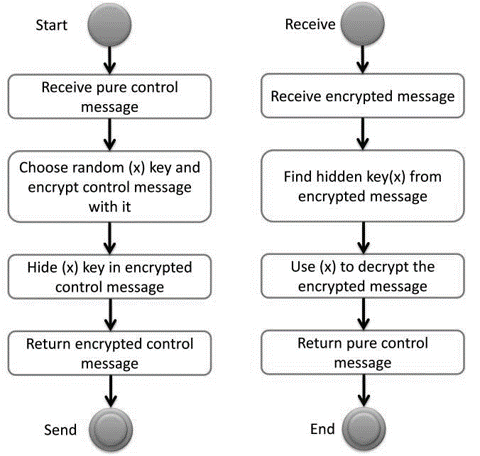
\includegraphics[scale=0.8]{gix.png}
%\caption{GIX Algorithm}
%\end{figure}
